\documentclass[a4paper,12pt]{article}
\usepackage[utf8]{inputenc}
\usepackage[T1]{fontenc}
\usepackage[includeheadfoot,margin=2cm]{geometry}
\usepackage{times}
\usepackage{booktabs}
\usepackage{enumitem}
\usepackage{amsmath}
\usepackage{mathptmx}
\usepackage{tikz}
\usepackage{xspace}
\frenchspacing
\setlist{nosep}
\renewcommand{\ttdefault}{cmtt}
\author{Thor Kristoffersen}
\date{\today}
\title{Guide to Building a Machine}
\newcommand{\num}[1]{\texttt{#1}\xspace}
\newcommand{\hex}[1]{\num{#1}$_{\textup{\tiny\hskip-1ex 16}}$\xspace}
\newcommand{\bin}[1]{\num{#1}$_{\textup{\tiny\hskip-1ex 2}}$\xspace}
\newcommand{\PC}{\textbf{program counter}\xspace}
\newcommand{\SP}{\textbf{stack pointer}\xspace}
\newcommand{\TERM}{\textbf{terminated}\xspace}
\newcommand{\F}{\bin{0}}
\newcommand{\T}{\bin{1}}
\newcommand{\range}[2]{\{#1,\ldots,#2\}}
\newcommand{\comment}[1]{\begin{quote}[\textit{#1}]\end{quote}}
\newcommand{\op}[1]{#1}
\newcommand{\EXIT}      [1]{\op{\hex{00}}}
\newcommand{\NOP}       [1]{\op{\hex{01}}}
\newcommand{\JUMP}      [1]{\op{\hex{02}}}
\newcommand{\JUMPZERO}  [1]{\op{\hex{03}}}
\newcommand{\SETSP}     [1]{\op{\hex{04}}}
\newcommand{\GETPC}     [1]{\op{\hex{05}}}
\newcommand{\GETSP}     [1]{\op{\hex{06}}}
\newcommand{\PUSHZ}     [1]{\op{\hex{07}}}
\newcommand{\PUSHB}     [1]{\op{\hex{08}}}
\newcommand{\PUSHS}     [1]{\op{\hex{09}}}
\newcommand{\PUSHI}     [1]{\op{\hex{0A}}}
\newcommand{\PUSHL}     [1]{\op{\hex{0B}}}
\newcommand{\SIGXB}     [1]{\op{\hex{0C}}}
\newcommand{\SIGXS}     [1]{\op{\hex{0D}}}
\newcommand{\SIGXI}     [1]{\op{\hex{0E}}}
\newcommand{\LOADB}     [1]{\op{\hex{10}}}
\newcommand{\LOADS}     [1]{\op{\hex{11}}}
\newcommand{\LOADI}     [1]{\op{\hex{12}}}
\newcommand{\LOADL}     [1]{\op{\hex{13}}}
\newcommand{\STOREB}    [1]{\op{\hex{14}}}
\newcommand{\STORES}    [1]{\op{\hex{15}}}
\newcommand{\STOREI}    [1]{\op{\hex{16}}}
\newcommand{\STOREL}    [1]{\op{\hex{17}}}
\newcommand{\ALLOCATE}  [1]{\op{\hex{18}}}
\newcommand{\DEALLOCATE}[1]{\op{\hex{19}}}
\newcommand{\ADD}       [1]{\op{\hex{20}}}
\newcommand{\MULT}      [1]{\op{\hex{21}}}
\newcommand{\DIV}       [1]{\op{\hex{22}}}
\newcommand{\REM}       [1]{\op{\hex{23}}}
\newcommand{\LT}        [1]{\op{\hex{24}}}
\newcommand{\AND}       [1]{\op{\hex{28}}}
\newcommand{\OR}        [1]{\op{\hex{29}}}
\newcommand{\NOT}       [1]{\op{\hex{2A}}}
\newcommand{\XOR}       [1]{\op{\hex{2B}}}
\newcommand{\POW}       [1]{\op{\hex{2C}}}
\newcommand{\NEWFRAME}  [1]{\op{\hex{30}}}
\newcommand{\SETPIXEL}  [1]{\op{\hex{31}}}
\newcommand{\ADDSAMPLE} [1]{\op{\hex{32}}}
\newcommand{\PUTCHAR}   [1]{\op{\hex{34}}}
\newcommand{\READFRAME} [1]{\op{\hex{38}}}
\newcommand{\READPIXEL} [1]{\op{\hex{39}}}

\newlist{stepnumbers}{enumerate}{2}
\setlist[stepnumbers]{label=\arabic*.}
\newlist{stepletters}{enumerate}{1}
\setlist[stepletters]{label=\alph*.}

\begin{document}

\maketitle

\noindent
This film contains programs that can be executed on a machine.
The purpose of this part of the film is to guide you through the process of building this machine.
To understand this guide, you need to have knowledge of basic 20th-century mathematics and physics.

You will start by building a very simple machine, and then you will extend this machine through several stages, so that by the end you will have a fully functional machine.

When you have finished the machine, you are not quite ready to run programs yet.
First you will need to install in the machine an initial program, which is supplied here.

\comment{Provide time estimates for the above tasks.}

\section{Building the Machine}
\label{sec:building-machine}

By following the instructions here, you can develop the machine through several stages, each stage leading to a more capable machine than the preceding one.
Only when you have obtained the correct test results for each stage should you proceed with the following stage.

Number systems used here include decimal, binary, and hexadecimal.
All non-decimal numbers are explictly indicated by subscripts indicating the number base in decimal.
Further detail on binary and hexadecimal notation can be found in Appendixes~\ref{sec:binary-notation} and \ref{sec:hexadecimal-notation}.

\subsection{Storage}

To build the machine, you first need storage to represent state consisting of binary digits (bits).
A storage \emph{element} is a group of bits forming a unit with respect to naming.
The number of bits in an element is called the \emph{size} of the element.
Each element has a unique name, so that it can be unambiguously referred to, and the contents can be retrieved or stored in one atomic operation.
This machine employs element sizes of 1, 8, and 64 bits.
The storage is divided into three categories:
\begin{description}
\item[Memory] 
The memory consists of a number of 8-bit elements, up to a maximum of $2^{64}$.
Each memory element is named by an integer in the range from $0$ to $2^{64} - 1$.
When testing the storage, and when building the first versions of the machine, we will limit the number of memory elements to $2^8$.
\item[Registers] 
There are two registers, named respectively the \PC and the \SP.
Both of these are 64-bit elements.
The contents of either register are interpreted as a non-negative integer referring to a memory element.
\item[Flags] 
There is one flag, named the \TERM flag, which is a 1-bit element.
\end{description}
In addition to the elements defined here, it is sometimes necessary to use additional elements temporarily.
These \emph{auxiliary} elements will be created and initialized whenever needed and are named by single letters.

\subsection{Storage Operations}
\label{sec:storage-operations}

We need to define a few terms to talk about storage operations.
\begin{itemize}
\item ``The value of an element'' means the contents as retrieved from that element.
\item ``To set the value of an element to $x$'' means to store the value of $x$ in that element.
\item ``To increment an element by $n$'' means to set the value of $x$ to the value of the element and then set that element to $(x + n) \mod 2^s$, where $s$ is the size of the element.
\item ``To decrement an element by $n$'' means to set the value of $x$ to the value of the element and then set that element to $(x - n) \mod 2^s$, where $s$ is the size of the element.
\item ``The value of \emph{octet} $i$ in $x$'' means the contents of the 8-bit subsequence of $x$ from bit number $8i+7$ to bit number $8i$.
\item ``To set \emph{octet} $i$ in $x$ to $y$'' means to store the 8-bit sequence $y$ in the 8-bit subsequence of $x$ from bit number $8i+7$ to bit number $8i$, while keeping all other bits of $x$ unchanged.
\end{itemize}
These should be basic operations in your implementation.

\subsection{Testing the Storage}

To test that the storage works as it should, do the following tests several times for every storage element:
\begin{stepnumbers}
\item Verify that storing and getting the value of an element works.
  \begin{stepletters}
  \item Select a random bit sequence, $x$, of the same size, $s$, as the storage element.
  \item Store this bit sequence in the element.
  \item Verify that the value of the element is $x$.
  \end{stepletters}
\item Verify that your operations for incrementing and decrementing an element work.
  \begin{stepletters}
  \item Select a random bit sequence, $n$, of size $s$, different from zero.
  \item Increment the element by $n$.
  \item Verify that the value of the element is $(x + n) \mod 2^s$.
  \item Decrement the element by $n$.
  \item Verify that the value of the element is $x$.
  \end{stepletters}
\item Verify that your octet operations work for every octet, $i$, from $0$ to $7$.
  \begin{stepletters}
  \item Get the value of all octets in $x$.
  \item Select a random bit sequence, $y$, of size $8$, different from the value of octet $i$.
  \item Set octet $i$ of the element to $y$.
  \item Verify that the value of octet $i$ is $y$.
  \item Verify that the values of all the other octets are unchanged.
  \end{stepletters}
\end{stepnumbers}

\subsection{Basic Procedures}

Some basic procedures are frequently used by the machine.
These use the storage operations in Section~\ref{sec:storage-operations}.

\subsubsection{Push Element}

Assume that we have an auxiliary 64-bit element called $x$.
The expression ``Push $x$'' means to do the following steps:
\begin{stepnumbers}
\item Initialize the auxiliary 8-bit element $i$ to 8.
\item Do the following 8 times:
  \begin{stepletters}
  \item Decrement $i$ by 1.
  \item Decrement \SP by 1.
  \item Set memory element \SP to octet $i$ of $x$.
  \end{stepletters}
\end{stepnumbers}

\subsubsection{Pop Element}

The expression ``Pop $x$'' means to do the following steps:
\begin{stepnumbers}
\item Initialize the auxiliary 64-bit element $x$ to 0.
\item Initialize the auxiliary 8-bit element $i$ to 0.
\item Do the following 8 times:
  \begin{stepletters}
  \item Set octet $i$ of $x$ to memory element \SP.
  \item Increment $i$ by 1.
  \item Increment \SP by 1.
  \end{stepletters}
\end{stepnumbers}
The 64-bit element $x$ can now be used by other procedures.

\subsubsection{Put Octets Into Memory}

Assume that we have two auxiliary 64-bit elements called $x$ and $a$, and that $n$ is either 1, 2, 4, or 8.
The expression ``Put $n$ octets from $x$ into memory at $a$'' means to do the following steps:
\begin{stepnumbers}
\item Initialize the auxiliary 8-bit element $i$ to 0.
\item Do the following $n$ times:
  \begin{stepletters}
  \item Set memory element $a+i$ to octet $i$ of $x$.
  \item Increment $i$ by 1.
  \end{stepletters}
\end{stepnumbers}

\subsubsection{Get Octets From Memory}

Assume that we have an auxiliary 64-bit element called $a$ and that $n$ is either 1, 2, 4, or 8.
The expression ``Get $n$ octets from memory at $a$ into $x$'' means to do the following steps:
\begin{stepnumbers}
\item Initialize the auxiliary 64-bit element $x$ to 0.
\item Initialize the auxiliary 8-bit element $i$ to 0.
\item Do the following $n$ times:
  \begin{stepletters}
  \item Set octet $i$ of $x$ to memory element $a+i$.
  \item Increment $i$ by 1.
  \end{stepletters}
\end{stepnumbers}
The auxiliary 64-bit element $x$ can now be used by other procedures.

\subsubsection{Fetch Octets}

Assume that $n$ is either 1, 2, 4, or 8.
The expression ``Fetch $n$ octets into $x$'' means to do the following steps:
\begin{stepnumbers}
\item Initialize the auxiliary 64-bit element $x$ to 0.
\item Initialize the auxiliary 8-bit element $i$ to 0.
\item Do the following $n$ times:
  \begin{stepletters}
  \item Set octet $i$ of $x$ to memory element \PC.
  \item Increment $i$ by 1.
  \item Increment \PC by 1.
  \end{stepletters}
\end{stepnumbers}
The auxiliary 64-bit element $x$ can now be used by other procedures.

\subsubsection{Sign Extend}

Assume that we have an auxiliary 64-bit element called $x$ and that $n$ is either 1, 2, or 4.
The expression ``Sign extend $n$ octets in $x$'' means to do the following:
\begin{stepnumbers}
\item If the value of bit $8n-1$ of $x$ is 1, then for all $i \in \range{8n}{63}$ set the value of bit $i$ of $x$ to 1, otherwise do nothing.
\end{stepnumbers}
The auxiliary 64-bit element $x$ can now be used by other procedures.

\subsection{Testing the Basic Procedures}

To test the basic procedures, do as follows:
\begin{stepnumbers}
\item Set \SP to \hex{0000000000000008}.
\item Initialize the auxiliary 64-bit element $x$ to \hex{0123456789ABCDEF}.
\item Push $x$.
\item Pop $y$.
\item Verify that $x=y$.
\item Verify that the value of \SP is \hex{0000000000000008}.
\item Verify that the contents of the first eight memory elements are as in the following table.
\end{stepnumbers}

\begin{center}
  \begin{tabular}{@{}lr@{}}
    \hline
    Storage element        & Value    \\
    \hline
    \hex{0000000000000000} & \hex{EF} \\
    \hex{0000000000000001} & \hex{CD} \\
    \hex{0000000000000002} & \hex{AB} \\
    \hex{0000000000000003} & \hex{89} \\
    \hex{0000000000000004} & \hex{67} \\
    \hex{0000000000000005} & \hex{45} \\
    \hex{0000000000000006} & \hex{23} \\
    \hex{0000000000000007} & \hex{01} \\
    \hline
  \end{tabular}
\end{center}

\comment{Test fetch, put, get, sign extend too.}

\subsection{First Version of The Machine}

You can now proceed with implementing a basic version of the machine.
For practical reasons we will build this version of the machine with $2^{8}$ memory elements.

Machine operation proceeds through two phases: first the storage is initialized, and then the main procedure is executed.

\subsubsection{Storage Initialization}

To initialize the storage, you need to set registers and flags to predefined values.
The \PC is set to $0$, and the \SP is set to the number of memory elements in the machine, that is, $2^{8}$ in this version of the machine.
The values are given in the table below.

\begin{center}
  \begin{tabular}{@{}lr@{}}
    \hline
    Register or flag & Value                   \\
    \hline
    \PC              & \hex{0000000000000000}  \\
    \SP              & \hex{0000000000000100}  \\
    \TERM            & \F                      \\
    \hline
  \end{tabular}
\end{center}

\subsubsection{The Main Procedure}

When you have initialized the storage, simply execute the main procedure repeatedly until the value of the \TERM flag is \T.
The main procedure must carry out the following steps.
\begin{stepnumbers}
\item Initialize the auxiliary 64-bit element $k$ to 0.
\item Fetch 1 octet into $k$.
\item\label{itm:main-case} If $k$ is
  \begin{description}
  \item[\EXIT{}] then set the value of \TERM to \T.
  \item[\NOP{}] then do nothing.
  \item[\JUMP{}] then
    \begin{stepnumbers}
    \item Initialize the auxiliary 64-bit element $a$ to 0.
    \item Pop $a$.
    \item Set \PC to $a$.
    \end{stepnumbers}
  \item[\JUMPZERO{}] then
    \begin{stepnumbers}
    \item Initialize the auxiliary 64-bit elements $a$ and $x$ to 0.
    \item Fetch 1 octet into $a$.
    \item Sign extend 1 octet in $a$.
    \item Pop $x$.
    \item If the value of $x$ is 0, then increment \PC by $a$, otherwise do nothing.
    \end{stepnumbers}
  \item[\SETSP{}] then
    \begin{stepnumbers}
    \item Initialize the auxiliary 64-bit element $a$ to 0.
    \item Pop $a$.
    \item Set \SP to $a$.
    \end{stepnumbers}
  \item[\GETPC{}] then
    \begin{stepnumbers}
    \item Initialize the auxiliary 64-bit element $a$ to \PC.
    \item Push $a$.
    \end{stepnumbers}
  \item[\GETSP{}] then
    \begin{stepnumbers}
    \item Initialize the auxiliary 64-bit element $a$ to \SP.
    \item Push $a$.
    \end{stepnumbers}
  \item[\PUSHL{}] then
    \begin{stepnumbers}
    \item Initialize the auxiliary 64-bit element $a$ to 0.
    \item Fetch 8 octets into $a$.
    \item Push $a$.
    \end{stepnumbers}
  \end{description}
\item If the value does not occur in the list above, abort and report an error.
\end{stepnumbers}

\subsubsection{Testing the Basic Machine}

To test the machine, first initialize all memory elements to the value \hex{00}, and then set the following memory elements to the provided values.

\begin{center}
  \begin{tabular}{@{}ll@{}}
    \hline
    Memory element         & Value \\
    \hline
    \hex{0000000000000000} & \hex{01} \\
    \hex{0000000000000001} & \hex{0B} \\
    \hex{0000000000000002} & \hex{13} \\
    \hex{0000000000000003} & \hex{00} \\
    \hex{0000000000000004} & \hex{00} \\
    \hex{0000000000000005} & \hex{00} \\
    \hex{0000000000000006} & \hex{00} \\
    \hex{0000000000000007} & \hex{00} \\
    \hex{0000000000000008} & \hex{00} \\
    \hex{0000000000000009} & \hex{00} \\
    \hex{000000000000000A} & \hex{02} \\
    \hex{000000000000000B} & \hex{00} \\
    \hex{000000000000000C} & \hex{00} \\
    \hex{000000000000000D} & \hex{00} \\
    \hex{000000000000000E} & \hex{00} \\
    \hex{000000000000000F} & \hex{00} \\
    \hline
  \end{tabular}
  \hfil
  \begin{tabular}{@{}ll@{}}
    \hline
    Memory element         & Value \\
    \hline
    \hex{0000000000000010} & \hex{00} \\
    \hex{0000000000000011} & \hex{00} \\
    \hex{0000000000000012} & \hex{00} \\
    \hex{0000000000000013} & \hex{06} \\
    \hex{0000000000000014} & \hex{05} \\
    \hex{0000000000000015} & \hex{0B} \\
    \hex{0000000000000016} & \hex{F8} \\
    \hex{0000000000000017} & \hex{00} \\
    \hex{0000000000000018} & \hex{00} \\
    \hex{0000000000000019} & \hex{00} \\
    \hex{000000000000001A} & \hex{00} \\
    \hex{000000000000001B} & \hex{00} \\
    \hex{000000000000001C} & \hex{00} \\
    \hex{000000000000001D} & \hex{00} \\
    \hex{000000000000001E} & \hex{04} \\
    \hex{000000000000001F} & \hex{00} \\
    \hline
  \end{tabular}
\end{center}

Now start the machine.
When it terminates, all storage elements should remain unchanged, except the following ones, which should have the indicated values.

\begin{center}
  \begin{tabular}{@{}lr@{}}
    \hline
    Storage element        & Value                   \\
    \hline
    \PC                    & \hex{0000000000000020}  \\
    \SP                    & \hex{00000000000000F8}  \\
    \TERM                  & \T                      \\
    \hex{00000000000000E8} & \hex{F8} \\
    \hex{00000000000000F0} & \hex{15} \\
    \hex{00000000000000F9} & \hex{01} \\
    \hline
  \end{tabular}
\end{center}

If the machine does not terminate or you did not get exactly the above results, the implementation is incorrect.

\comment{Test \JUMPZERO{} too.}

\subsection{Second Version of the Machine}

In the next version of the machine you will add several more cases to step \ref{itm:main-case} of the main procedure.

\begin{stepnumbers}[start=3]
\item If $k$ is
  \begin{description}
  \item[\LOADL{}] then
    \begin{stepnumbers}
    \item Initialize the auxiliary 64-bit elements $a$ and $x$ to 0.
    \item Pop $a$.
    \item Get 8 octets from memory at $a$ into $x$.
    \item Push $x$.
    \end{stepnumbers}
  \item[\STOREL{}] then
    \begin{stepnumbers}
    \item Initialize the auxiliary 64-bit elements $a$ and $x$ to 0.
    \item Pop $a$.
    \item Pop $x$.
    \item Put 8 octets from $x$ into memory at $a$.
    \end{stepnumbers}
  \item[\ADD{}] then
    \begin{stepnumbers}
    \item Pop the 64-bit value $y$.
    \item Pop the 64-bit value $x$.
    \item Push the 64-bit value $(x + y) \mod 2^{64}$.
    \end{stepnumbers}
  \item[\MULT{}] then
    \begin{stepnumbers}
    \item Initialize the auxiliary 64-bit elements $x$ and $y$ to 0.
    \item Pop $y$.
    \item Pop $x$.
    \item Push $x y \mod 2^{64}$.
    \end{stepnumbers}
  \item[\DIV{}] then
    \begin{stepnumbers}
    \item Initialize the auxiliary 64-bit elements $x$ and $y$ to 0.
    \item Pop $y$.
    \item Pop $x$.
    \item If $x > 0$ and $y > 0$, then push $q$, such that $x = qy + r$ and $0 \leq r < y$, otherwise push 0.
    \end{stepnumbers}
  \item[\REM{}] then
    \begin{stepnumbers}
    \item Initialize the auxiliary 64-bit elements $x$ and $y$ to 0.
    \item Pop $y$.
    \item Pop $x$.
    \item If $x > 0$ and $y > 0$, then push $r$, such that $x = qy + r$ and $0 \leq r < y$, otherwise push 0.
    \end{stepnumbers}
  \item[\LT{}] then
    \begin{stepnumbers}
    \item Initialize the auxiliary 64-bit elements $x$ and $y$ to 0.
    \item Pop $y$.
    \item Pop $x$.
    \item If $x < y$, then push $2^{64} - 1$, otherwise push 0.
    \end{stepnumbers}
  \item[\AND{}] then
    \begin{stepnumbers}
    \item Initialize the auxiliary 64-bit elements $x$, $y$, and $z$ to 0.
    \item Pop $y$.
    \item Pop $x$.
    \item For every $i \in \range{0}{63}$, if bit $i$ of $x$ is 1 and bit $i$ of $y$ is 1, then set bit $i$ of $z$ to 1, otherwise, set bit $i$ of $z$ to 0.
    \item Push $z$.
    \end{stepnumbers}
  \item[\OR{}] then
    \begin{stepnumbers}
    \item Initialize the auxiliary 64-bit elements $x$, $y$, and $z$ to 0.
    \item Pop $y$.
    \item Pop $x$.
    \item For every $i \in \range{0}{63}$, if bit $i$ of $x$ is 0 and bit $i$ of $y$ is 0, then set bit $i$ of $z$ to 0, otherwise, set bit $i$ of $z$ to 1. %
    \item Push $z$.
    \end{stepnumbers}
  \item[\NOT{}] then
    \begin{stepnumbers}
    \item Initialize the auxiliary 64-bit elements $x$ and $z$ to 0.
    \item Pop $x$.
    \item For every $i \in \range{0}{63}$, if bit $i$ of $x$ is 1, then set bit $i$ of $z$ to 0, otherwise set bit $i$ of $z$ to 1.
    \item Push $z$.
    \end{stepnumbers}
  \item[\XOR{}] then
    \begin{stepnumbers}
    \item Initialize the auxiliary 64-bit elements $x$, $y$, and $z$ to 0.
    \item Pop $y$.
    \item Pop $x$.
    \item For every $i \in \range{0}{63}$, if bit $i$ of $x$ is different from bit $i$ of $y$, then set bit $i$ of $z$ to 1, otherwise set bit $i$ of $z$ to 0.
    \item Push the 64-bit value $z$.
    \end{stepnumbers}
  \item[\POW{}] then
    \begin{stepnumbers}
    \item Initialize the auxiliary 64-bit element $x$ to 0.
    \item Pop $x$.
    \item If $x < 64$, then push $2^x$, otherwise push 0.
    \end{stepnumbers}
  \end{description}
\end{stepnumbers}

\comment{More tests here.}

\subsection{Third Version of the Machine}

In the third version of the machine you will add still more cases to step \ref{itm:main-case} of the main procedure.

\begin{stepnumbers}[start=3]
\item If $k$ is
  \begin{description}
  \item[\PUSHB{}] then
    \begin{stepnumbers}
    \item Initialize the auxiliary 64-bit element $a$ to 0.
    \item Fetch 1 octet into $a$.
    \item Push $a$.
    \end{stepnumbers}
  \item[\PUSHS{}] then
    \begin{stepnumbers}
    \item Initialize the auxiliary 64-bit element $a$ to 0.
    \item Fetch 2 octets into $a$.
    \item Push $a$.
    \end{stepnumbers}
  \item[\PUSHI{}] then
    \begin{stepnumbers}
    \item Initialize the auxiliary 64-bit element $a$ to 0.
    \item Fetch 4 octets into $a$.
    \item Push $a$.
    \end{stepnumbers}
  \item[\SIGXB{}] then
    \begin{stepnumbers}
    \item Initialize the auxiliary 64-bit element $x$ to 0.
    \item Pop $x$.
    \item Sign extend 1 octet in $x$.
    \item Push $x$.
    \end{stepnumbers}
  \item[\SIGXS{}] then
    \begin{stepnumbers}
    \item Initialize the auxiliary 64-bit element $x$ to 0.
    \item Pop $x$.
    \item Sign extend 2 octets in $x$.
    \item Push $x$.
    \end{stepnumbers}
  \item[\SIGXI{}] then
    \begin{stepnumbers}
    \item Initialize the auxiliary 64-bit element $x$ to 0.
    \item Pop $x$.
    \item Sign extend 4 octets in $x$.
    \item Push $x$.
    \end{stepnumbers}
  \item[\LOADB{}] then
    \begin{stepnumbers}
    \item Initialize the auxiliary 64-bit element $a$ to 0.
    \item Pop $a$.
    \item Get 1 octet from memory at $a$ into $x$.
    \item Push $x$.
    \end{stepnumbers}
  \item[\LOADS{}] then
    \begin{stepnumbers}
    \item Initialize the auxiliary 64-bit element $a$ to 0.
    \item Pop $a$.
    \item Get 2 octets from memory at $a$ into $x$.
    \item Push $x$.
    \end{stepnumbers}
  \item[\LOADI{}] then
    \begin{stepnumbers}
    \item Initialize the auxiliary 64-bit element $a$ to 0.
    \item Pop $a$.
    \item Get 4 octets from memory at $a$ into $x$.
    \item Push $x$.
    \end{stepnumbers}
  \item[\STOREB{}] then
    \begin{stepnumbers}
    \item Initialize the auxiliary 64-bit elements $a$ and $x$ to 0.
    \item Pop $a$.
    \item Pop $x$.
    \item Put 1 octet from $x$ into memory at $a$.
    \end{stepnumbers}
  \item[\STORES{}] then
    \begin{stepnumbers}
    \item Initialize the auxiliary 64-bit elements $a$ and $x$ to 0.
    \item Pop $a$.
    \item Pop $x$.
    \item Put 2 octets from $x$ into memory at $a$.
    \end{stepnumbers}
  \item[\STOREI{}] then
    \begin{stepnumbers}
    \item Initialize the auxiliary 64-bit elements $a$ and $x$ to 0.
    \item Pop $a$.
    \item Pop $x$.
    \item Put 4 octets from $x$ into memory at $a$.
    \end{stepnumbers}
  \item[\ALLOCATE{}] then
    \begin{stepnumbers}
    \item Initialize the 64-bit element $n$ and $a$ to 0.
    \item Pop $n$.
    \item Create a new range of $n$ new memory elements.
    \item Set $a$ to the integer that names the first element in the range.
    \item Push $a$.
    \end{stepnumbers}
  \item[\DEALLOCATE{}] then
    \begin{stepnumbers}
    \item Initialize the 64-bit element $a$ to 0.
    \item Pop $a$.
    \item Discard the range of memory elements whose first element is $a$.
    \end{stepnumbers}
  \end{description}
\end{stepnumbers}

\comment{More tests here.}

\section{Building the Devices}
\label{sec:building-devices}

At this point you should have a machine with fully functional computational capabilities.
What's missing are the devices that allow the machine to consume data from its environment and to produce data to its environment.
There are four devices:
\begin{itemize}
\item The \emph{Image Input} device allows the machine to consume images as a two-dimensional matrix of gray-scale values.
  This device is very important, because it is what enables the machine to load programs encoded as images on the film.
\item The \emph{Image Output} device allows the machine to produce color images.
  Moving images are supported by producing a time series of still images.
\item The \emph{Audio Output} device allows the machine to produce audio signals as a time series of amplitude values.
\item The \emph{Text Output} device allows the machine to produce text as a stream of characters.
\end{itemize}
The descriptions below will only explain the correspondence between machine events and real world events.
It is up to you to make sure that the interpretation of real world events is faithfully implemented.

\subsection{Image Input}

The \emph{Image Input} device allows the machine to consume an image as a two-dimensional matrix of points of light intensity values.
The following figure shows an example of such a matrix, consisting of 32 sampling points arranged in 8 columns and 4 rows.
\begin{center}
  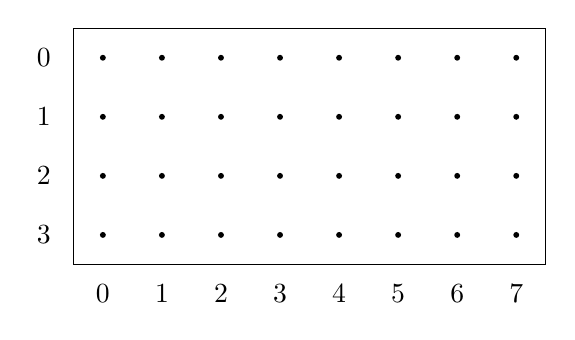
\begin{tikzpicture}[scale=0.75]
    \foreach \x in {0,...,7}
    \foreach \y in {0,...,3}
    {
      \fill (\x,\y) circle [radius=0.5mm,fill=black,draw] {};
    }
    \foreach \x in {0,...,7} \draw (\x, -1) node {\x};
    \foreach \y in {0,...,3} \draw (-1, 3 - \y) node {\y};
    \draw (-0.5,-0.5) -- (7.5,-0.5) -- (7.5,3.5) -- (-0.5,3.5) -- cycle;
  \end{tikzpicture}
\end{center}
As shown, both columns and rows are numbered consecutively, starting at 0.
The spacing between the sampling points must be uniform in both horizontal and vertical directions, and an anti-aliasing filter must be employed to limit the bandwidth of the image to satisfy the Nyquist-Shannon sampling theorem.

Each picture element detects the intensity of light transmitted or reflected at a sampling point in that particular position of the image, represented as one of 256 intensity levels, from 0 (minimum intensity) to 255 (maximum intensity).
Values between 0 and 255 represent intermediate intensities between these extremes.

\comment{I'm not sure how much of this should be explained in this document or elsewhere.}

In order to implement the image input device, you will need to add two extra cases to step \ref{itm:main-case} of the main procedure.

\begin{stepnumbers}[start=3]
\item If $k$ is
  \begin{description}
  \item[\READFRAME{}] then
    \begin{stepnumbers}
    \item Initialize the auxiliary 64-bit elements $c$ and $r$ to 0.
    \item Ready the next image to be consumed by the machine, and measure the intensity of light at all sampling points.
    \item Set the value of $c$ to the number of columns in the image.
    \item Push $c$.
    \item Set the value of $r$ to the number of rows in the image.
    \item Push $r$.
    \end{stepnumbers}
  \item[\READPIXEL{}] then
    \begin{stepnumbers}
    \item Initialize the auxiliary 64-bit elements $x$ and $y$ to 0.
    \item Pop $x$.
    \item Pop $y$.
    \item Find the intensity of light in the image at column $x$ and row $y$, represented as an 8-bit value, $z$.
    \item Decrement \SP.
    \item Set the value of memory element \SP to $z$.
    \end{stepnumbers}
  \end{description}
\end{stepnumbers}

\subsection{Image Output}

The \emph{Image Output} device allows the machine to produce an image represented as a two-dimensional matrix of points of color space values.
Moving images can be produced as a sequence of images.

In order to implement the image output device, you will need to add two extra cases to step \ref{itm:main-case} of the main procedure.

\begin{stepnumbers}[start=3]
\item If $k$ is
  \begin{description}
  \item[\NEWFRAME{}] then
    \begin{stepnumbers}
    \item Finish and render the frame constructed so far.
    \item Initialize the auxiliary 64-bit elements $r$, $w$, and $h$ to 0.
    \item Pop $r$.
    \item Pop $h$.
    \item Pop $w$.
    \item Set the frame rate to $r$, the width of the frame to $w$, and the height of the frame to $h$.
    \end{stepnumbers}
  \item[\SETPIXEL{}] then
    \begin{stepnumbers}
    \item Initialize the auxiliary 64-bit elements  $x$, $y$, $r$, $g$, and $b$, to 0.
    \item Pop $b$.
    \item Pop $g$.
    \item Pop $r$.
    \item Pop $y$.
    \item Pop $x$.
    \item Set the picture element at column $x$ and row $y$ to the point in the color space represented by the tuple $(r,g,b)$.
    \end{stepnumbers}
  \end{description}
\end{stepnumbers}

\subsection{Audio Output}

The \emph{Audio Output} device allows the machine to produce two-channel audio signal represented as a series of magnitude values.

In order to implement the audio output device, you will need to add one extra case to step \ref{itm:main-case} of the main procedure.

\begin{stepnumbers}[start=3]
\item If $k$ is
  \begin{description}
  \item[\NEWFRAME{}] then
    \begin{stepnumbers}
    \item Initialize the auxiliary 64-bit elements  $l$ and $r$ to 0.
    \item Pop $r$.
    \item Pop $l$.
    \item Set the audio signal magnitude of the left channel to $l$.
    \item Set the audio signal magnitude of the right channel to $r$.
    \end{stepnumbers}
  \end{description}
\end{stepnumbers}

\subsection{Text Output}

In order to implement the text output device, you will need to add one extra case to step \ref{itm:main-case} of the main procedure.

\begin{stepnumbers}[start=3]
  \setcounter{enumi}{2}
\item If $k$ is
  \begin{description}
  \item[\PUTCHAR{}] then
    \begin{stepnumbers}
    \item Initialize the auxiliary 64-bit element $c$ to 0.
    \item Pop $c$.
    \item Produce the character with Unicode code point $c$.
    \end{stepnumbers}
  \end{description}
\end{stepnumbers}

\section{Installing the Initial Program}

\appendix

\section{Binary Notation}
\label{sec:binary-notation}

Each storage element contains a binary value, that is, a sequence of binary digits that can be retrieved or modified in one atomic operation.

In this documentation, individual binary digits are referred to using non-negative integers, listed in decreasing order.
For an $n$-bit value, the individual bits, $b_i$, are numbered as follows:
\[ b_{n-1} \; b_{n-2} \; \ldots \; b_{1} \; b_{0} \]
Bit $n-1$ is called the most significant bit (MSB), and bit 0 is called the least significant bit (LSB).
For example,
\begin{itemize}
\item in the 4-bit element \bin{0001}, bit number 0 (or LSB) is 1, and
\item in the 4-bit element \bin{1000}, bit number 3 (or MSB) is 1.
\end{itemize}

When an $n$-bit binary element is interpreted as a non-negative integer, the value of that integer is
\[
    v = \sum_{i=0}^{n-1} b_{i}2^{i}
\]

\section{Hexadecimal Notation}
\label{sec:hexadecimal-notation}

For convenience, binary numbers are normally written in hexadecimal notation.
Each hexadecimal digit corresponds to a group of four binary digits, as shown in the following table.

\begin{center}
  \begin{tabular}{@{}ll@{}}
    \hline
    Hexadecimal digit & Group of binary digits \\
    \hline
    \num{0}           & \num{0000}   \\
    \num{1}           & \num{0001}   \\
    \num{2}           & \num{0010}   \\
    \num{3}           & \num{0011}   \\
    \num{4}           & \num{0100}   \\
    \num{5}           & \num{0101}   \\
    \num{6}           & \num{0110}   \\
    \num{7}           & \num{0111}   \\
    \num{8}           & \num{1000}   \\
    \num{9}           & \num{1001}   \\
    \num{A}           & \num{1010}   \\
    \num{B}           & \num{1011}   \\
    \num{C}           & \num{1100}   \\
    \num{D}           & \num{1101}   \\
    \num{E}           & \num{1110}   \\
    \num{F}           & \num{1111}   \\
    \hline
  \end{tabular}
\end{center}

\section{The Initial Program}
\label{sec:initial-program}

\comment{Include a listing in hex of the initial program.}
\end{document}
